\documentclass[]{article}
\usepackage{lmodern}
\usepackage{amssymb,amsmath}
\usepackage{ifxetex,ifluatex}
\usepackage{fixltx2e} % provides \textsubscript
\ifnum 0\ifxetex 1\fi\ifluatex 1\fi=0 % if pdftex
  \usepackage[T1]{fontenc}
  \usepackage[utf8]{inputenc}
\else % if luatex or xelatex
  \ifxetex
    \usepackage{mathspec}
    \usepackage{xltxtra,xunicode}
  \else
    \usepackage{fontspec}
  \fi
  \defaultfontfeatures{Mapping=tex-text,Scale=MatchLowercase}
  \newcommand{\euro}{€}
\fi
% use upquote if available, for straight quotes in verbatim environments
\IfFileExists{upquote.sty}{\usepackage{upquote}}{}
% use microtype if available
\IfFileExists{microtype.sty}{%
\usepackage{microtype}
\UseMicrotypeSet[protrusion]{basicmath} % disable protrusion for tt fonts
}{}
\usepackage[margin=1in]{geometry}
\usepackage{longtable,booktabs}
\ifxetex
  \usepackage[setpagesize=false, % page size defined by xetex
              unicode=false, % unicode breaks when used with xetex
              xetex]{hyperref}
\else
  \usepackage[unicode=true]{hyperref}
\fi
\hypersetup{breaklinks=true,
            bookmarks=true,
            pdfauthor={Andrés Herrera Poyatos, Antonio Rafael Moya Martín-Castaño, Iván Sevillano García, Juan Luis Suárez Díaz},
            pdftitle={Algorítmica: Práctica 1},
            colorlinks=true,
            citecolor=blue,
            urlcolor=blue,
            linkcolor=magenta,
            pdfborder={0 0 0}}
\urlstyle{same}  % don't use monospace font for urls
\setlength{\parindent}{0pt}
\setlength{\parskip}{6pt plus 2pt minus 1pt}
\setlength{\emergencystretch}{3em}  % prevent overfull lines
\setcounter{secnumdepth}{0}

%%% Use protect on footnotes to avoid problems with footnotes in titles
\let\rmarkdownfootnote\footnote%
\def\footnote{\protect\rmarkdownfootnote}

%%% Change title format to be more compact
\usepackage{titling}

% Create subtitle command for use in maketitle
\newcommand{\subtitle}[1]{
  \posttitle{
    \begin{center}\large#1\end{center}
    }
}

\setlength{\droptitle}{-2em}
  \title{Algorítmica: Práctica 1}
  \pretitle{\vspace{\droptitle}\centering\huge}
  \posttitle{\par}
  \author{Andrés Herrera Poyatos, Antonio Rafael Moya Martín-Castaño, Iván
Sevillano García, Juan Luis Suárez Díaz}
  \preauthor{\centering\large\emph}
  \postauthor{\par}
  \date{}
  \predate{}\postdate{}

\usepackage{graphicx}


\begin{document}

\maketitle


\subsection{Organización de la
práctica}\label{organizacion-de-la-practica}

Se adjunta el directorio comprimido \textbf{code} con todos los datos
obtenidos. La información se organiza como sigue:

\begin{itemize}
\itemsep1pt\parskip0pt\parsep0pt
\item
  Los códigos \textbf{.cpp} de los distintos algoritmos están
  disponibles en la carpeta \textbf{src}.
\item
  Se añade el script de bash \textbf{ejecuciones.sh}, el cual se encarga
  de obtener todos los datos y gráficas para todos los algoritmos.
\item
  En la carpeta \textbf{sh} se añaden scripts auxiliares, cada uno
  especializado en la toma de datos de uno o varios algoritmos
  concretos.
\item
  En la carpeta \textbf{plot}, de la misma forma, se encuentran scripts
  especializados en la elaboración de las distintas gráficas.
\item
  En las carpetas \textbf{Datos\emph{Autor}} se almacenan los archivos
  .dat generados por cada uno de los autores, en sus respectivos PCs.
  Los ficheros contienen, para cada algoritmo, varias parejas
  \emph{{[}tamaño tiempo{]}} correspondientes a distintas ejecuciones
  del programa con distintos tamaños y sus respectivos resultados. con
  los datos utilizados en el trabajo.
\item
  De forma análoga, están disponibles los directorios
  \textbf{Tablas\emph{Autor}} e \textbf{Imagenes\emph{Autor}} que
  contienen tablas en formato \textbf{.md} con los resultados, y las
  gráficas del comportamiento de los algoritmos generadas por
  \emph{gnuplot}, respectivamente.
\end{itemize}

Cada ejercicio tiene su apartado en el pdf con su corresponiente
enunciado y solución.

\textbf{\emph{Nota:}} Se ha utilizado el shell bash para la obtención de
los distintos datos de los algoritmos.

\subsection{Ejercicio 1: Cálculo de la eficiencia
empírica}\label{ejercicio-1-calculo-de-la-eficiencia-empirica}

Calcule la eficiencia empírica de los algoritmos pedidos. Defina
adecuadamente los tamaños de entrada para que se generen al menos 25
datos. Incluya en la memoria tablas diferentes para los algoritmos de
distinto orden de eficiencia (una con los algoritmos \(O(n^2)\), otra
con los \(O(n \log{n})\), otra con \(O(n^3)\) y otra con
\(O((\frac{1+\sqrt{5}}{2})^n)\).

A continuación se disponen las distintas tablas para cada clase de
algoritmos:

\subsubsection{Tabla con los algoritmos
cuadráticos}\label{tabla-con-los-algoritmos-cuadraticos}

\begin{longtable}[c]{@{}llll@{}}
\toprule
Tamaño del Vector & Burbuja & Seleccion & Insercion\tabularnewline
\midrule
\endhead
1000 & 0.005971 & 0.003397 & 0.001321\tabularnewline
2000 & 0.018136 & 0.009589 & 0.007588\tabularnewline
3000 & 0.024143 & 0.014704 & 0.020282\tabularnewline
4000 & 0.043267 & 0.025817 & 0.023064\tabularnewline
5000 & 0.067684 & 0.037817 & 0.034221\tabularnewline
6000 & 0.099499 & 0.055028 & 0.047872\tabularnewline
7000 & 0.137072 & 0.073739 & 0.064517\tabularnewline
8000 & 0.181558 & 0.092111 & 0.082905\tabularnewline
9000 & 0.232648 & 0.118624 & 0.103043\tabularnewline
10000 & 0.290489 & 0.14394 & 0.124546\tabularnewline
11000 & 0.354349 & 0.178614 & 0.151216\tabularnewline
12000 & 0.433737 & 0.20678 & 0.178228\tabularnewline
13000 & 0.519202 & 0.239558 & 0.209278\tabularnewline
14000 & 0.59308 & 0.273397 & 0.248141\tabularnewline
15000 & 0.689312 & 0.314147 & 0.276967\tabularnewline
16000 & 0.789129 & 0.356495 & 0.317291\tabularnewline
17000 & 0.890449 & 0.402106 & 0.358508\tabularnewline
18000 & 1.01538 & 0.450575 & 0.397242\tabularnewline
19000 & 1.1313 & 0.50472 & 0.435913\tabularnewline
20000 & 1.26128 & 0.55525 & 0.483853\tabularnewline
21000 & 1.39441 & 0.611367 & 0.541654\tabularnewline
22000 & 1.55788 & 0.670662 & 0.600085\tabularnewline
23000 & 1.68169 & 0.732809 & 0.644882\tabularnewline
24000 & 1.84769 & 0.800821 & 0.70273\tabularnewline
25000 & 1.9893 & 0.864984 & 0.762199\tabularnewline
\bottomrule
\end{longtable}

\subsubsection{Tabla con los algoritmos
cúbicos}\label{tabla-con-los-algoritmos-cubicos}

\begin{longtable}[c]{@{}ll@{}}
\toprule
Nodos del Grafo & Floyd\tabularnewline
\midrule
\endhead
32 & 0.000596\tabularnewline
64 & 0.004593\tabularnewline
96 & 0.01017\tabularnewline
128 & 0.017141\tabularnewline
160 & 0.035407\tabularnewline
192 & 0.054113\tabularnewline
224 & 0.083649\tabularnewline
256 & 0.116013\tabularnewline
288 & 0.153556\tabularnewline
320 & 0.217792\tabularnewline
352 & 0.280357\tabularnewline
384 & 0.362685\tabularnewline
416 & 0.460287\tabularnewline
448 & 0.581175\tabularnewline
480 & 0.703839\tabularnewline
512 & 0.852424\tabularnewline
544 & 1.02124\tabularnewline
576 & 1.25977\tabularnewline
608 & 1.44669\tabularnewline
640 & 1.68365\tabularnewline
672 & 1.93344\tabularnewline
704 & 2.23303\tabularnewline
736 & 2.54158\tabularnewline
768 & 2.89293\tabularnewline
800 & 3.25971\tabularnewline
\bottomrule
\end{longtable}

\subsubsection{Tabla con el algoritmo de Fibonacci
(\(O((\frac{1+\sqrt{5}}{2})^n)\))}\label{tabla-con-el-algoritmo-de-fibonacci-ofrac1sqrt52n}

\begin{longtable}[c]{@{}ll@{}}
\toprule
Índice & Fibonacci\tabularnewline
\midrule
\endhead
15 & 1.3e-05\tabularnewline
16 & 2e-05\tabularnewline
17 & 2.6e-05\tabularnewline
18 & 4.4e-05\tabularnewline
19 & 5e-05\tabularnewline
20 & 0.000114\tabularnewline
21 & 8.6e-05\tabularnewline
22 & 0.000154\tabularnewline
23 & 0.000582\tabularnewline
24 & 0.00097\tabularnewline
25 & 0.001314\tabularnewline
26 & 0.002554\tabularnewline
27 & 0.002394\tabularnewline
28 & 0.003356\tabularnewline
29 & 0.004289\tabularnewline
30 & 0.007083\tabularnewline
31 & 0.011583\tabularnewline
32 & 0.017354\tabularnewline
33 & 0.029313\tabularnewline
34 & 0.047371\tabularnewline
35 & 0.073093\tabularnewline
36 & 0.127835\tabularnewline
37 & 0.190808\tabularnewline
38 & 0.308124\tabularnewline
39 & 0.498824\tabularnewline
40 & 0.849934\tabularnewline
\bottomrule
\end{longtable}

\subsubsection{Tabla con el algoritmo de Hanoi
(\(O(2^n))\))}\label{tabla-con-el-algoritmo-de-hanoi-o2n}

\begin{longtable}[c]{@{}ll@{}}
\toprule
Num. Discos & Hanoi\tabularnewline
\midrule
\endhead
5 & 1e-06\tabularnewline
6 & 3e-06\tabularnewline
7 & 3e-06\tabularnewline
8 & 6e-06\tabularnewline
9 & 9e-06\tabularnewline
10 & 1.3e-05\tabularnewline
11 & 4.9e-05\tabularnewline
12 & 7.6e-05\tabularnewline
13 & 0.00015\tabularnewline
14 & 0.00019\tabularnewline
15 & 0.000393\tabularnewline
16 & 0.000851\tabularnewline
17 & 0.002302\tabularnewline
18 & 0.003382\tabularnewline
19 & 0.009191\tabularnewline
20 & 0.019015\tabularnewline
21 & 0.024593\tabularnewline
22 & 0.041194\tabularnewline
23 & 0.065421\tabularnewline
24 & 0.127555\tabularnewline
25 & 0.246427\tabularnewline
26 & 0.483075\tabularnewline
27 & 0.96832\tabularnewline
28 & 1.9249\tabularnewline
29 & 3.83247\tabularnewline
30 & 7.63996\tabularnewline
\bottomrule
\end{longtable}

\subsubsection{Tabla con los algoritmos n log
n}\label{tabla-con-los-algoritmos-n-log-n}

\begin{longtable}[c]{@{}lll@{}}
\toprule
Tamaño del Vector & Mergesort & Quicksort\tabularnewline
\midrule
\endhead
40000 & 0.015087 & 0.006235\tabularnewline
80000 & 0.02682 & 0.014736\tabularnewline
120000 & 0.037756 & 0.02246\tabularnewline
160000 & 0.041266 & 0.025439\tabularnewline
200000 & 0.059359 & 0.032775\tabularnewline
240000 & 0.057706 & 0.041055\tabularnewline
280000 & 0.065938 & 0.045861\tabularnewline
320000 & 0.082393 & 0.053183\tabularnewline
360000 & 0.093771 & 0.057395\tabularnewline
400000 & 0.107337 & 0.063843\tabularnewline
440000 & 0.102685 & 0.071064\tabularnewline
480000 & 0.122825 & 0.076521\tabularnewline
520000 & 0.136037 & 0.082585\tabularnewline
560000 & 0.141045 & 0.087434\tabularnewline
600000 & 0.150005 & 0.093448\tabularnewline
640000 & 0.1658 & 0.100634\tabularnewline
680000 & 0.181068 & 0.109131\tabularnewline
720000 & 0.211107 & 0.115456\tabularnewline
760000 & 0.205422 & 0.121493\tabularnewline
800000 & 0.226734 & 0.129283\tabularnewline
840000 & 0.200972 & 0.136155\tabularnewline
880000 & 0.211482 & 0.141553\tabularnewline
920000 & 0.23571 & 0.148845\tabularnewline
960000 & 0.240497 & 0.155352\tabularnewline
1000000 & 0.244299 & 0.178312\tabularnewline
\bottomrule
\end{longtable}

Finalmente, mostramos una tabla con la comparativa de todos los
algoritmos de ordenación, tanto cuadráticos como \(n \log{n}\). Podemos
apreciar, que para tamaños relativamente pequeños (25.000), ya se
muestran diferencias bastante grandes:

\subsubsection{Tabla con los algoritmos de
ordenación}\label{tabla-con-los-algoritmos-de-ordenacion}

\begin{longtable}[c]{@{}llllll@{}}
\toprule
Tamaño del Vector & Burbuja & Seleccion & Insercion & Mergesort &
Quicksort\tabularnewline
\midrule
\endhead
1000 & 0.005971 & 0.003397 & 0.001321 & 0.000359 &
0.000195\tabularnewline
2000 & 0.018136 & 0.009589 & 0.007588 & 0.000756 &
0.000269\tabularnewline
3000 & 0.024143 & 0.014704 & 0.020282 & 0.00074 &
0.000671\tabularnewline
4000 & 0.043267 & 0.025817 & 0.023064 & 0.000748 &
0.00067\tabularnewline
5000 & 0.067684 & 0.037817 & 0.034221 & 0.002255 &
0.000567\tabularnewline
6000 & 0.099499 & 0.055028 & 0.047872 & 0.001549 &
0.001661\tabularnewline
7000 & 0.137072 & 0.073739 & 0.064517 & 0.003041 &
0.001953\tabularnewline
8000 & 0.181558 & 0.092111 & 0.082905 & 0.003166 &
0.002456\tabularnewline
9000 & 0.232648 & 0.118624 & 0.103043 & 0.004058 &
0.001649\tabularnewline
10000 & 0.290489 & 0.14394 & 0.124546 & 0.003803 &
0.001971\tabularnewline
11000 & 0.354349 & 0.178614 & 0.151216 & 0.004144 &
0.002048\tabularnewline
12000 & 0.433737 & 0.20678 & 0.178228 & 0.0041 & 0.003616\tabularnewline
13000 & 0.519202 & 0.239558 & 0.209278 & 0.005279 &
0.003037\tabularnewline
14000 & 0.59308 & 0.273397 & 0.248141 & 0.006677 &
0.002399\tabularnewline
15000 & 0.689312 & 0.314147 & 0.276967 & 0.006024 &
0.002247\tabularnewline
16000 & 0.789129 & 0.356495 & 0.317291 & 0.007461 &
0.002721\tabularnewline
17000 & 0.890449 & 0.402106 & 0.358508 & 0.006324 &
0.002745\tabularnewline
18000 & 1.01538 & 0.450575 & 0.397242 & 0.008806 &
0.005765\tabularnewline
19000 & 1.1313 & 0.50472 & 0.435913 & 0.008887 & 0.004034\tabularnewline
20000 & 1.26128 & 0.55525 & 0.483853 & 0.007868 &
0.003407\tabularnewline
21000 & 1.39441 & 0.611367 & 0.541654 & 0.00544 & 0.00359\tabularnewline
22000 & 1.55788 & 0.670662 & 0.600085 & 0.006238 &
0.00374\tabularnewline
23000 & 1.68169 & 0.732809 & 0.644882 & 0.010339 &
0.006076\tabularnewline
24000 & 1.84769 & 0.800821 & 0.70273 & 0.010512 &
0.006921\tabularnewline
25000 & 1.9893 & 0.864984 & 0.762199 & 0.009398 &
0.003104\tabularnewline
\bottomrule
\end{longtable}

\subsection{Ejercicio 2: Elaboración de
gráficas.}\label{ejercicio-2-elaboracion-de-graficas.}

Con cada una de las tablas anteriores, genere un gráfico comparando los
tiempos de los algoritmos. Indique claramente el significado de cada
serie. Para los algoritmos que realizan la misma tarea (los de
ordenación), incluya también una gráfica con todos ellos, para poder
apreciar las diferencias de rendimiento de algoritmos con diferente
orden de eficiencia.

\subsubsection{Gráfica comparativa de los algoritmos
cuadráticos.}\label{grafica-comparativa-de-los-algoritmos-cuadraticos.}

\(\centerline{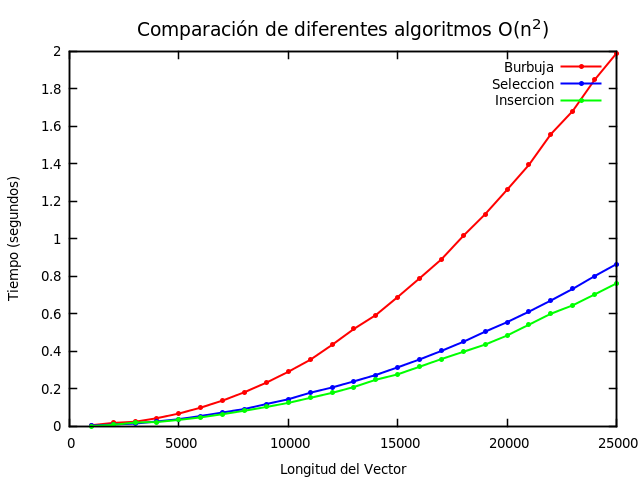
\includegraphics[height=7cm]{./Code/ImagenesAndres/cuadraticos.png}}\)

\subsubsection{Gráfica del algoritmo cúbico
(Floyd)}\label{grafica-del-algoritmo-cubico-floyd}

\(\centerline{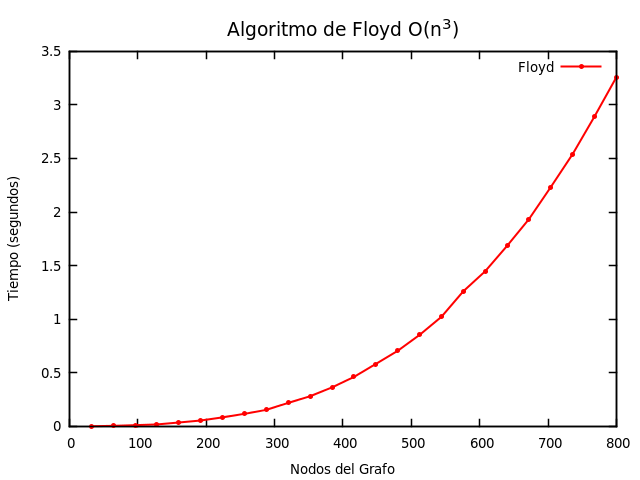
\includegraphics[height=7cm]{./Code/ImagenesAndres/cubicos.png}}\)

\subsubsection{Gráfica del algoritmo de Fibonacci
(\(O((\frac{1+\sqrt{5}}{2})^n)\))}\label{grafica-del-algoritmo-de-fibonacci-ofrac1sqrt52n}

\(\centerline{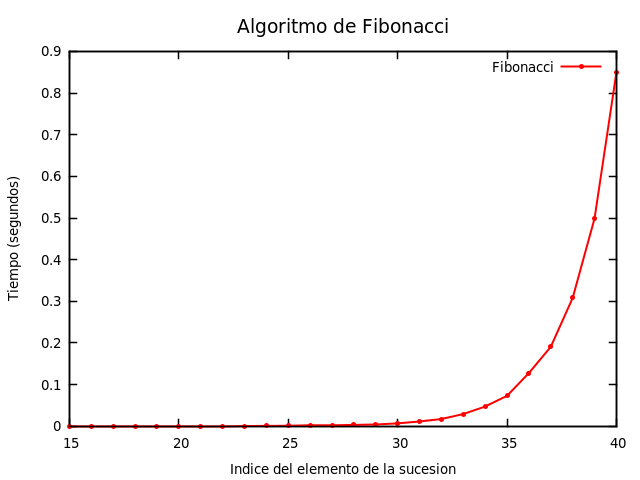
\includegraphics[height=7cm]{./Code/ImagenesAndres/fibonacci.png}}\)

\subsubsection{Gráfica del algoritmo de Hanoi
(\(O(2^n)\))}\label{grafica-del-algoritmo-de-hanoi-o2n}

\(\centerline{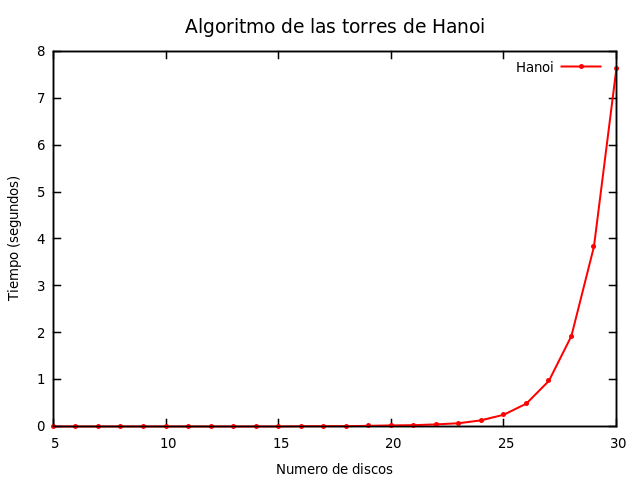
\includegraphics[height=7cm]{./Code/ImagenesAndres/hanoi.png}}\)

\subsubsection{Gráfica de los algoritmos
\(O(n \log{n})\)}\label{grafica-de-los-algoritmos-on-logn}

\(\centerline{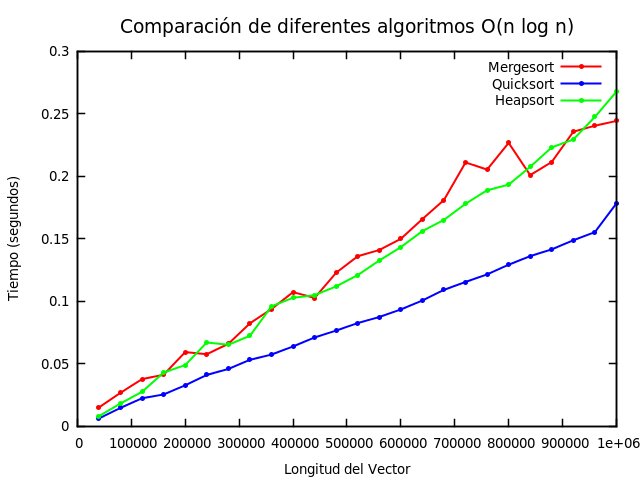
\includegraphics[height=7cm]{./Code/ImagenesAndres/nlogn.png}}\)

\subsubsection{Gráfica comparativa con todos los algoritmos de
ordenación.}\label{grafica-comparativa-con-todos-los-algoritmos-de-ordenacion.}

\(\centerline{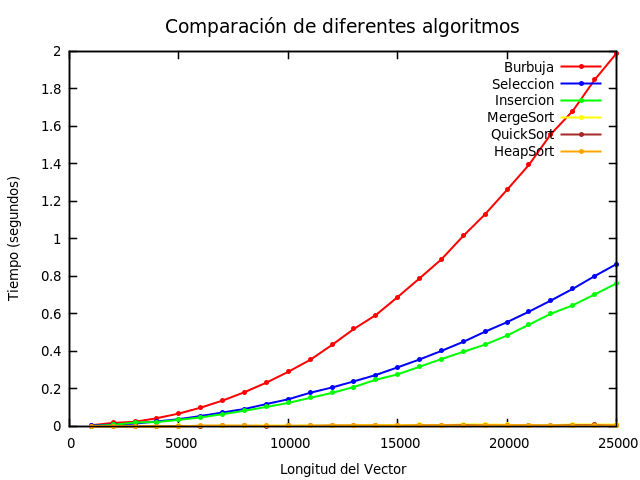
\includegraphics[height=7cm]{./Code/ImagenesAndres/ordenacion.png}}\)

\end{document}
